\section{Introduction}
\label{sec:intro}

Large language models (LLMs) ~\cite{brown2020language, touvron2023llama, zeng2022glm, zhang2022opt, touvron2023llama2} demonstrate significant capabilities.
Besides delivering online LLM services~\cite{cai, chatgpt, AmazonCode, GithubCopilot}, there remain important scenarios where strict latency SLO constraints are unnecessary, such as batch APIs~\cite{openai-batch-api, anyscale-batch-api} and RLHF rollout stage~\cite{hu2024openrlhfeasytousescalablehighperformance}.
In these offline settings, maximizing the throughput has become the top priority.
However, given the substantial memory demands of LLMs and a single GPU's capacity is often insufficient, existing approaches~\cite{sheng2023flexgen, 2022deepspeed, shoeybi2019megatron, huang2019gpipe, dudu2024liger} cannot effectively coordinate multiple resources with minimal synchronization overhead for high-throughput LLM inference.

LLM generative inference entails substantial memory requirements and requires different resources to cooperate.
On the one hand, LLMs are renowned for their massive weights.
The number of parameters can be 7B, 13B, 30B, 70B, 175B, and so on, taking up tens or even hundreds of gigabytes.
On the other hand, LLM generative tasks require storing a large amount of KV cache, often exceeding the memory consumed by the weights, so as to enable sufficient parallelism and saturate GPU resources~\cite{yu2022orca, agrawal2024taming, zhong2024distserve, lee2024infinigen}.
To meet the requirement in terms of large memory, existing systems typically employ offloading or parallel approaches.


\begin{figure}[!t]
    \centering
    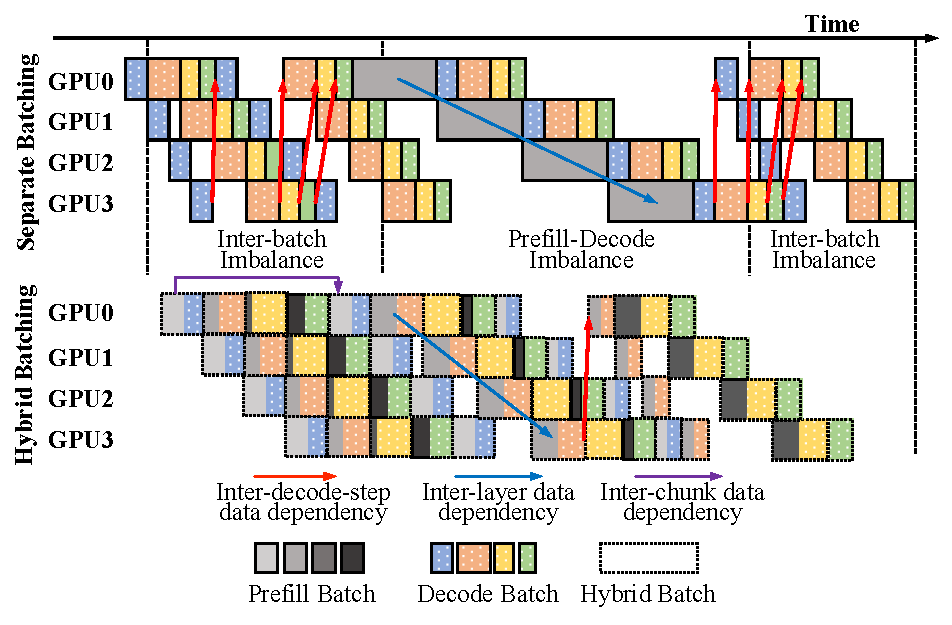
\includegraphics[width=0.95\linewidth]{fig/pipeline_bubble.pdf}
    \caption{Bubbles in LLM pipeline parallel inference.}
    \label{fig:pipeline_bubble}
    \vspace{-10pt}
\end{figure}
Offloading approaches run an LLM with limited GPU memory by offloading data to the secondary storage and retrieving it when the data is accessed. 
By carefully optimizing the computation schedule and tensor placement, existing offloading approaches~\cite{sheng2023flexgen, 2022deepspeed} can hide data transfer between GPU memory and the secondary storage with computation, achieving considerable throughput on each GPU.
Unfortunately, offloading approaches inherently suffer from severe contention problems.
Specifically, under the commonly-used multi-GPU architecture, several GPUs share the only one channel linked with CPU, and consequently there is serious bandwidth contention on CPU’s root complexes when multiple GPUs offload data simultaneously.

Parallel approaches distribute a single LLM inference instance across multiple devices.
Tensor parallelism~\cite{shoeybi2019megatron, dudu2024liger} is widely used in existing LLM serving systems~\cite{nvidia2023fast, 2022deepspeed, vllm2024, tensorrt2024} due to its simplicity.
Through splitting each layer into symmetric fragments and distributing fragments, devices performs the similar computation, and they communicate with collective primitives, following the single program multiple data (SPMD) model.
However, due to the frequent and intensive synchronizations, considerable communication overhead makes it inefficient.


In comparison, pipeline parallelism~\cite{huang2019gpipe, dudu2024liger} splits a model by layers and only transfers activations between cut-off layers.
This low-communication feature makes it a promising approach for fully exploiting the computational capabilities of devices.
However, due to the imbalanced pipeline workloads and complex data dependencies, achieving compact scheduling is challenging, and bubbles always exist.
Figure~\ref{fig:pipeline_bubble} presents the running process of batching prefill and decode phases separately and scheduling them in an interleaved manner, as in most practical LLM inference systems~\cite{vllm2024, tensorrt2024,zheng2024sglang}.
The imbalanced workloads come from two aspects.
First, different batch sizes lead to different decode step workloads, resulting in the inter-batch imbalance.
Second, the prefill-decode imbalance exists as the execution of prefill usually takes much longer time than a decode step. 
Likewise, the data dependencies also come from two aspects.
On the one hand, inter-layer data dependency requires data to be processed in the current layer before entering to the next layer for processing.
On the other hand, inter-decode-step data dependency exists as the execution of generating the next token cannot start until the previous iteration completes.


\begin{figure}[!t]
    \centering
    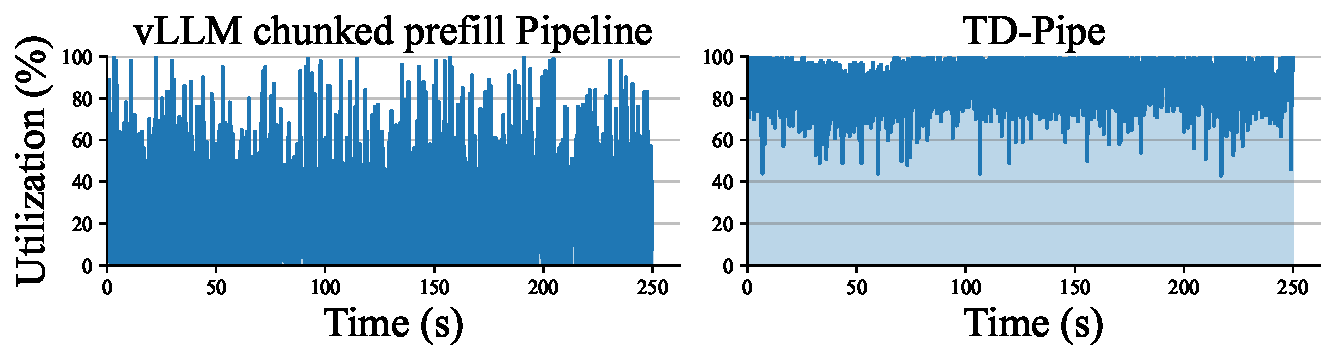
\includegraphics[width=0.95\linewidth]{fig/GPUse.pdf}
    \caption{GPU Utilization in Pipeline Parallelism.}
    \label{fig:gpu_usage}
    \vspace{-10pt}
\end{figure}

An alternative approach to mitigate the pipeline bubble problem is the combination of the chunked-prefill approach~\cite{agrawal2024taming} and the hybrid batching~\cite{yu2022orca}. 
Chunked prefill is now commonly used in many LLM serving systems to balance TTFT and TPOT.
By splitting the prefill computation into chunks and mixing these chunks with decode, chunked prefill can achieve better inter-batch load balance.
However, 1) it depends on the prefill-to-decode ratio and struggles to handle requests with continuously varying lengths, 2) it introduces tighter data dependency as prefills are mixed with decodes and chunks of a single prefill introduce new data dependency, 3)it incurs repeated KV cache loading overhead.
The lower part of Figure~\ref{fig:pipeline_bubble} illustrates how its bubbles emerge even when starting from an initially balanced pipeline.
Over time, complex data dependencies and the continuous arrival and completion of requests exacerbate this issue.
To better illustrate its inefficiency, the left part of Figure~\ref{fig:gpu_usage} shows that it suffers from significant GPU underutilization.
Therefore, existing pipeline parallelism approaches always suffer from severe bubble problems.

To better leverage pipeline parallelism for high-throughput LLM inference, we propose TD-Pipe, an LLM inference system based on the temporally-disaggregated pipeline parallelism architecture. Its key idea is to disaggregate the prefill and decode phases in the temporal dimension, or rather, to reduce the prefill-decode switching frequency as much as possible.
Thus, load balance between pipeline stages can be effectively maintained in prefill and decode phases respectively and data dependency can be largely resolved.
As shown in right part of Figure~\ref{fig:gpu_usage}, TD-Pipe significantly improves GPU utilization.


We further identify key challenges in supporting this novel architecture and provides solutions.
It includes a hierarchy-controller system structure and three novel approaches.
The hierarchy-controller architecture enables asynchronous device coordination in a pipeline.
Since different devices perform consecutive layers of a model and LLM inference workloads are generally irregular in terms of input and output lengths, the device-to-device transfer has to be in a blocking style.
The hierarchy-controller decouples the scheduling from execution by introducing the distributed runtime (execution plane) and the centralized engine (control plane), enabling unblocked transmission.

Next, we present three approaches to further enhance the temporal disaggregation benefit.
First, to delay the timing of switching from prefill to decode and perform more prefills, we propose the AI-based greedy prefill approach.
To prevent it from exceeding the memory capacity, we leverage the output length prediction model.
As some requests will finish and the related KV cache is freed during decoding, we can perform prefills more aggressively with length prediction. 
Second, to reduce pipeline bubbles in the decode phase, we propose the inter-batch work stealing approach.
Since requests will finish randomly and result in imbalance, this approach dynamically balances the number of requests between batches.
Third, to determine the optimal timing of switching from decode back to prefill, we propose the spatial-temporal intensity comparison approach.
As decode progresses, some requests complete, leading to a gradual drop in computational intensity, this is referred to as spatial intensity.
Meanwhile, switching to the decode phase introduces pipeline bubbles, and the proportion of time the hardware is effectively utilized is defined as temporal intensity.
By comparing them, we identify the switching point.
In summary, we make the following contributions:
\begin{itemize}[leftmargin=*]
    \item We identify causes of bubble problem in LLM generative tasks when using the pipeline parallelism. 
    \item We design the novel temporally-disaggregated pipeline parallelism architecture targeting at throughput-oriented offline LLM inference, which disaggregates the prefill and decode phases in the temporal dimension.
    \item We identify potential issues with the exploitation of novel architecture and present TD-Pipe with three approaches.
    \item We evaluate TD-Pipe and show its efficiency.
\end{itemize}